\documentclass{article}  

\usepackage{times}
\usepackage{graphicx}
\usepackage{lipsum}  
\usepackage{xcolor}
\usepackage{fullpage}
\usepackage{url}
\usepackage{amsmath}
\usepackage{caption}
\usepackage{float}
\usepackage{listings}
\usepackage{xcolor}

\lstdefinelanguage{Cypher}{
  morekeywords={MATCH, WITH, WHERE, RETURN, ORDER, BY, LIMIT, AS,
                 DESC, ASC, AND, OR, IN, DISTINCT, COUNT, SUM, AVG,
                 ROUND, CASE, WHEN, THEN, END, COLLECT, UNWIND},
  sensitive=true,
  morecomment=[l]{//},
}

\lstdefinestyle{cypherstyle}{
  language=Cypher,
  basicstyle=\ttfamily\small,
  keywordstyle=\bfseries,
  commentstyle=\normalfont,
  backgroundcolor=\color{white},
  frame=single,
  framerule=0.4pt,
  rulecolor=\color{black},
  breaklines=true,
  breakatwhitespace=false,
  columns=flexible,
  xleftmargin=2pt,
  xrightmargin=2pt,
  framexleftmargin=5pt,
  framexrightmargin=5pt,
}
\newcommand{\question}[1]{#1}

\title{Knowledge Graph for Culinary Sustainability and User Engagement Analysis}
\author{Varshini Ramakrishnan (2265001), Abitha Bala Subramani (2257963), \\
Martin Demirev (2276224), Harish Venkatramanan (2292068)}

\begin{document}
\date{\today}
\maketitle

This datasheet was prepared following the ``Datasheets for Datasets'' template of Gebru et al.\ \cite{gebru}, extended where needed following the frameworks of Pushkarna et al.\ \cite{pushkarna} and Paullada et al.\ \cite{Paullada}.

%%%%%%%%%%%%%%%%%%%%%%%%%%%%%%%%%%%%%%%%%%%%%%%%%%%%%%%%%%%%%%%%%%%%%%%%%%%%%%%%
\section{Motivation For Data/Knowledge Creation}

\question{\subsubsection*{Why was the dataset/knowledge graph created? (e.g., was there a specific task in mind? was there a specific gap that needed to
be filled?)}}

The development of this Knowledge Graph was to address the operational requirements of the client, NutriSmart, a consultancy specialized in the sustainability optimization of commercial restaurant menus. The primary objective is to engineer a system capable of generating ``eco scores" for complex recipes, thereby providing consumers with transparent, data-driven insights into the environmental footprint of their food choices. Currently, a significant technical gap exists because the necessary data, comprising culinary recipes, ingredient-specific emissions, and user engagement metrics are distributed across disparate and disconnected datasets. Furthermore, existing culinary datasets often suffer from naming inconsistencies that prevent accurate mapping to environmental impact values. This Knowledge Graph was designed specifically to resolve these discrepancies.

\question{\subsubsection*{What (other) tasks could the dataset be used for?}}


Beyond the primary objective of automated ``eco-score" generation, the integrated Knowledge Graph provides a robust foundation for several advanced analytical and operational tasks:

\begin{itemize}
    \item \textbf{Explainable Sustainability Analysis:} The graph-based architecture enables the decomposition of a recipe's total environmental footprint, allowing users to pinpoint specific high-impact ingredients that contribute disproportionately to the overall carbon range.
    \item \textbf{User Preference and Engagement Correlation:} By synthesizing historical interaction data from recipe dataset with environmental metrics, the system can investigate whether recipe-level sustainability scores significantly influence user ratings or community engagement patterns over time.
    \item \textbf{Culinary Pattern Recognition and Trend Mining:} The Knowledge Graph facilitates the discovery of top-N co-occurring ingredient pairs within high-carbon recipes, offering quantitative insights into culinary trends that drive greenhouse gas emissions.
    \item \textbf{Menu Optimization and Ingredient Substitution:} The system establishes a scalable infrastructure for NutriSmart to suggest lower-impact ingredient alternatives while maintaining recipe coherence, thereby assisting restaurants in aligning with institutional sustainability standards.
\end{itemize}


\question{\subsubsection*{Research Questions}}

The analytical scope of the Knowledge Graph is defined by three research questions (RQs):

\begin{enumerate}
    \item[\textbf{RQ1}] Which ingredients contribute most significantly to recipe-level carbon footprint ranges, and how frequently do these ingredients appear in the top-$k$ highly rated recipes?
    \item[\textbf{RQ2}] What top-$N$ co-occurring ingredient pairs and their average CO$_2$e contribution emerge among the top-$k$ high-carbon recipes?
    \item[\textbf{RQ3}] Do recipes with higher estimated carbon footprints differ in their nutritional profile (calories, protein, fat, sugar) compared to low-carbon recipes, and does this trade-off between nutritional density and environmental impact relate to user engagement?
\end{enumerate}

\question{\subsubsection*{Any other comments?}}
The selection of a Knowledge Graph as the primary data structure is a strategic choice dictated by the highly interconnected nature of the domains involved. This will allow for flexible relationship traversal that traditional relational models cannot adequately support.


\section{Dataset and Knowledge Graph Composition}

\question{\subsubsection*{What do the instances that comprise the dataset represent? (e.g., documents, images, people, countries) Are there multiple types of instances? (e.g., movies, users, ratings; people, interactions between them; nodes, edges)}}

In the Knowledge Graph, the instances represent a structured synthesis of regional culinary heritage and environmental impact metrics. Rather than a collection of flat documents, the dataset is comprised of heterogeneous entities that define a specialised ``Sustainability Knowledge Layer'':
\begin{itemize}
    \item \textbf{Recipes:} Central nodes representing unique South Asian culinary compositions (e.g., Sajji, Dal Makhani, Sindhi Biryani). Each instance serves as a container for master metadata, including cuisine origin, difficulty level, and meal type.
    \item \textbf{Ingredients:} Canonical food items extracted from recipe compositions (e.g., Paneer, Ghee, Chickpeas). These are modelled as discrete entities with associated attributes such as culinary category and mass-normalised quantities.
    \item \textbf{Environmental Impact Factors:} Quantitative instances derived from two scientific sources. Primary CO$_2$e values come from the Wolfram Food Carbon Footprint dataset (538 foods, compiled from peer-reviewed LCA studies including Poore \& Nemecek 2018). For 4 ingredients absent from Wolfram, fallback values were sourced from the Our World in Data GHG Emissions per kg dataset (Poore \& Nemecek 2018 via OWID). Each instance is a CO$_2$e rate (kg CO$_2$e/kg of food) mapped to a canonical ingredient entity.
    \item \textbf{Gram-Weight Conversion References:} 4,446 portion entries from the USDA FoodData Central SR Legacy database (2018 release), each providing an empirically measured gram weight for a specific food item and culinary unit (e.g., tablespoon, teaspoon, cup, medium). These entries are used during preprocessing to convert recipe quantity strings into metric mass (grams) before CO$_2$e calculation. USDA data does not itself become a node in the Knowledge Graph --- it enriches the \texttt{HAS\_INGREDIENT} edge with a \texttt{grams} attribute derived from the conversion.
    \item \textbf{Nutritional Components:} Discrete instances of macro and micronutrients (e.g., protein, fibre, iron) associated with each recipe, representing the physiological value of the culinary instance.
\end{itemize}


There are multiple types of instances.The dataset is architected as a heterogeneous knowledge graph consisting of various node and edge types. This multi-modal structure allows for complex traversal across different data domains:
\begin{itemize}
    \item \textbf{Nodes (Entity Instances):} The graph (built in \texttt{ingest\_desktop.py})
    contains four distinct classes of nodes:
    \begin{itemize}
        \item \textit{Recipe Nodes:} Master entities containing high-level metadata, ratings,
        denormalised nutritional attributes, and the derived \texttt{total\_co2e} and
        \texttt{carbon\_tier} properties added by inference rule R1.
        \item \textit{Ingredient Nodes:} Building blocks of the recipes, each carrying its
        canonical CO$_2$e emission factor (\texttt{co2\_kg\_per\_kg}) and \texttt{usda\_tier}.
        \item \textit{Cuisine Nodes:} Organizational instances used for regional classification
        (e.g., Pakistani, Indian, Bangladeshi).
        \item \textit{NutritionalProfile Nodes:} One per recipe, holding the macro- and
        micronutrient attributes (calories, protein, fat, sugar, fibre, etc.).
    \end{itemize}
    \item \textbf{Edges (Relationship Instances):} The graph utilizes three directed
    relationship types to link these nodes:
    \begin{itemize}
        \item \textit{HAS\_INGREDIENT (Recipe $\rightarrow$ Ingredient):} A weighted relationship
        representing the inclusion of an ingredient, qualified by \texttt{grams} (the quantity in
        metric mass, grounded via USDA SR Legacy portion data), \texttt{co2e\_kg} (the ingredient's
        contribution to the recipe footprint), and \texttt{usda\_tier} (grounding provenance).
        \item \textit{BELONGS\_TO\_CUISINE (Recipe $\rightarrow$ Cuisine):} A semantic edge mapping
        each recipe to its regional cuisine.
        \item \textit{HAS\_NUTRITION (Recipe $\rightarrow$ NutritionalProfile):} A one-to-one edge
        connecting each recipe to its physiological profile.
    \end{itemize}
    The ingredient-to-carbon mapping is represented as a node property
    (\texttt{Ingredient.co2\_kg\_per\_kg}) rather than a separate node, and ingredient food
    categories are not modelled as nodes in the current schema.
\end{itemize}

\question{\subsubsection*{How many instances are there in total (of each type, if appropriate)?}}

The Knowledge Graph is comprised of a multi-modal collection of instances distributed
across culinary, nutritional, and environmental domains. The total population of instances
by type is detailed below:

\begin{itemize}
    \item \textbf{Recipe Nodes:} 9,997 unique South Asian recipes, each serving as a
    master node within the graph.
    \item \textbf{Ingredient Nodes:} 58 canonical entities, each associated with a
    validated CO$_2$e rate.
    \item \textbf{Cuisine Nodes:} 5 primary regional categories (Indian,
    Pakistani, Bangladeshi, Afghan, Fusion).
    \item \textbf{NutritionalProfile Nodes:} 9,997 instances, one per recipe,
    containing macro and micronutrient attributes.
    \item \textbf{HAS\_INGREDIENT Edges:} 96,139 directed edges. These are formed by
    merging the 103,908 ingredient line items on the (recipe, ingredient) pair, so
    repeated mentions of the same ingredient within a recipe collapse to a single edge.
    Each edge carries \texttt{grams}, \texttt{co2e\_kg}, and \texttt{usda\_tier} attributes.
    \item \textbf{BELONGS\_TO\_CUISINE Edges:} 9,997 directed edges linking each recipe
    to its cuisine.
    \item \textbf{HAS\_NUTRITION Edges:} 9,997 directed edges linking each recipe to its
    NutritionalProfile node.
    \item \textbf{CO$_2$e Factor Instances:} 58 validated emission rates
    (kg~CO$_2$e/kg of food), stored as a property on each canonical ingredient node.
    \item \textbf{Gram-Weight Conversion References (preprocessing only):} 4,446
    USDA SR Legacy portion entries used during pipeline execution; not stored as
    graph nodes.
\end{itemize}

In total, the Knowledge Graph manages approximately 20,000 nodes (9,997 Recipe,
9,997 NutritionalProfile, 58 Ingredient, 5 Cuisine) and approximately 116,000
relational edges (96,139 HAS\_INGREDIENT, 9,997 BELONGS\_TO\_CUISINE, 9,997
HAS\_NUTRITION) across culinary, nutritional, and environmental domains.

\question{\subsubsection*{What data does each instance consist of ? “Raw” data (e.g., unprocessed text or images)? Features/attributes? Is there a label/target associated with
instances? If the instances related to people, are subpopulations identified (e.g., by age, gender, etc.) and what is
their distribution?}}

The dataset consists of a combination of raw, unstructured text and highly structured features/attributes distributed across multiple relational tables:
\begin{itemize}
    \item \textbf{Raw Data (Unprocessed Text):} Natural language strings such as recipe\_name (e.g., "Sindhi Biryani"), ingredient\_name (e.g., "Fenugreek Leaves", "Paneer"), and step\_description (e.g., "Soak rice in water for 20 minutes").
    \item \textbf{Categorical Attributes:} Features such as cuisine (e.g., Pakistani, Fusion), category (e.g., Main Course), cooking\_method (e.g., Baked, Fried), difficulty (e.g., Easy, Hard), spice\_level (e.g., Mild), and meal\_type.
    \item \textbf{Numerical Features:} Quantitative attributes including temporal data (prep\_time\_minutes, cook\_time\_minutes), engagement metrics (rating, review\_count) and granular nutritional metrics (example calories, protein\_g, fat\_g, sodium\_mg, etc).
    \item \textbf{Boolean/Binary Features:} True/False flags indicating specific dietary and cultural classifications, specifically: is\_vegetarian, is\_vegan, is\_gluten\_free, is\_halal, is\_traditional, and is\_festival\_special.
\end{itemize}

\textbf{Is there a label/target associated with instances?} \\
Because the primary objective of this Knowledge Graph is exploratory analysis and semantic querying rather than supervised predictive modeling, the raw data does not contain a predefined "ground truth" label. However, based on the project's explicit research questions, specific instances are associated with the following designated target variables for analysis:

\begin{itemize}
    \item \textbf{Derived Environmental Target (Eco-Score):} To answer Research Questions
    1, 2, and 3, the primary analytical target is the \textbf{Recipe-Level Environmental
    Impact Score} (kg~CO$_2$eq per recipe). This is not a raw label but an engineered
    target calculated as:
    $\text{co2e\_kg} = \sum_{i} \bigl(\text{qty\_amount}_i \times \text{g\_per\_unit}_i
    \times \text{co2\_kg\_per\_kg}_i / 1000 \bigr)$,
    aggregating the CO$_2$e contributions of all matched ingredient instances.
    \item \textbf{User Preference Target:} To answer Research Question 1 (filtering the "top $k$ highly rated recipes") and Research Question 3 (associating environmental impact with user preference), the continuous feature \textbf{\textit{rating}} functions as the explicit target variable representing user sentiment.
    \item \textbf{Relational Targets (Co-occurrence):} To answer Research Question 2, the target of the graph traversal is the frequency count and average $CO_2e$ contribution of top-N ingredient pairs, which serves as the quantitative output of the recipe instance analysis.
\end{itemize}

\textbf{Subpopulation Identification and Distribution} \\
The instances in this dataset represent culinary entities (recipes, ingredients, nutritional profiles) and do not contain demographic information regarding human users. Consequently, human subpopulations based on age, gender, or socioeconomic status are not identified, and there is no human demographic distribution to report. Instead, the data identifies cultural subpopulations via cuisine origin: Indian
(35\%), Pakistani (30\%), Bangladeshi (15\%), Afghan (10\%), and Fusion (10\%).


\question{\subsubsection*{Is any information missing from individual instances? If so, please provide a description, explaining why this information is missing (e.g., because it was unavailable). This does not include intentionally removed information, but might include, e.g., redacted text.}}

Certain instances contain missing or incomplete data, primarily stemming from the inherent variability of natural language culinary records and the limitations of existing scientific databases:

\begin{itemize}
    \item \textbf{Non-Standardised Quantity Metrics:} A portion of ingredient instances lack precise mass or volume measurements. Entries such as ``to taste'', ``1 medium'', or ``handful'' provide no standardised numerical value. This information is missing because culinary data is historically recorded for human instruction rather than scientific precision. In the pipeline, irreducible qualitative quantities are assigned conservative fixed defaults (e.g., ``to taste'' $\approx$ 5g) and flagged in the \texttt{usda\_tier} column as \texttt{generic}.
    \item \textbf{Regional Environmental Impact Specificity:} Direct CO$_2$e emission factors for specialised South Asian ingredients --- specifically regional spice blends, traditional processed oils (Ghee), and local cultivations --- are absent from global LCA datasets. This gap exists due to the predominant focus of environmental research on Western agricultural staples, necessitating proxy mappings (e.g., Ghee mapped to Butter; Paneer mapped to Cheese via OWID).
    \item \textbf{Anonymised Interaction Metadata:} The dataset lacks demographic and geographic identifiers for the individuals who generated the ratings and review counts. This omission reflects the scope of the original data collection, which prioritised recipe attributes over user-profile metadata.
\end{itemize}


\question{\subsubsection*{Are relationships between individual instances made explicit (e.g.,
users’ movie ratings, social network links)? If so, please describe
how these relationships are made explicit.}}


The relationships between individual instances in the knowledge graph are made explicit through a relational schema using standardized unique identifiers and categorical mapping. These linkages define the structural connectivity of the South Asian culinary dataset:

\begin{itemize}
    \item \textbf{Recipe-Ingredient Composition:} Relationships between recipe instances and their constituent ingredients are explicitly defined in \texttt{recipe\_ingredients.csv}. The recipe\_id functions as a foreign key that links the master recipe node to multiple ingredient entries, each qualified by a quantity and ingredient\_number attribute.
    \item \textbf{Nutritional Attribution:} A one-to-one explicit relationship exists between recipes and their physiological data in \texttt{recipe\_nutrition.csv}. The recipe\_id ensures that each recipe node is directly associated with its specific macro and micronutrient attributes.
    \item \textbf{Categorical and Regional Hierarchy:} Individual recipes are explicitly linked to their broader cultural subpopulations through the cuisine attribute in \texttt{recipes\_master.csv}. This establishes a hierarchical relationship between specific dish instances and regional metadata (e.g., Pakistani, Afghan).
    \item \textbf{Sustainability Semantic Linkage:} In the final knowledge graph architecture, the relationship between an ingredient\_name and its environmental impact factor ($kg\ CO_2e/kg$) is made explicit via entity resolution. This allows for the traversal from a high-level recipe instance down to its calculated carbon footprint.
\end{itemize}

\question{\subsubsection*{Does the dataset contain all possible instances or is it a sample (not
necessarily random) of instances from a larger set (bootstrapping)? If the dataset is
a sample, then what is the larger set? Is the sample representative of the
larger set (e.g., geographic coverage)? If so, please describe how this
representativeness was validated/verified. If it is not representative of the
larger set, please describe why not (e.g., to cover a more diverse range of
instances, because instances were withheld or unavailable).}}

The dataset constitutes a \textbf{curated sample} rather than a universal collection of all possible South Asian culinary instances. It comprises 9,997 distinct recipes, which represent a significant subset of the broader South Asian "Culinary Corpus." The larger set from which this sample is drawn includes the vast, multi-millennial array of regional variations, family traditions, and undocumented recipes across the Indian subcontinent. The sample is designed to be \textbf{regionally representative} of the South Asian landmass. This representativeness is achieved through a stratified distribution across five major cultural nodes: Indian (35\%), Pakistani (30\%), Bangladeshi (15\%), Afghan (10\%), and Fusion (10\%). This ensures that the Knowledge Graph captures a diverse range of dietary patterns.
\\
 \newline By auditing the \textit{cuisine\_metadata.csv}, it was verified that each regional subpopulation contains a balanced distribution of meal types (e.g., Street Food, Main Course, Desserts) that correspond to the actual culinary prominence of those categories within the respective cultures. Although it represents the major traditions, the sample is not exhaustive regarding hyper-local or indigenous tribal cuisines. These instances were omitted primarily due to digital unavailability and a strategic project scope.

\question{\subsubsection*{Are there recommended data splits (e.g., training, development/validation, testing)? If so, please provide a description of these splits, explaining the rationale behind them.}}

No data splits were applied. The Knowledge Graph is constructed from the complete set of 9,997 recipe instances without partitioning into training, validation, or testing subsets. The analytical tasks (RQ1, RQ2, RQ3) are addressed through SPARQL queries over the full graph rather than through predictive model evaluation, so held-out partitions are not methodologically appropriate.


\question{\subsubsection*{Are there any errors, sources of noise, or redundancies in the dataset? If so, please provide a description.}}

The South Asian recipe dataset exhibited several forms of structural and semantic noise that required rigorous preprocessing:

\begin{itemize}
    \item \textbf{High-Cardinality Ingredient Redundancy (resolved):} The raw \texttt{recipe\_ingredients.csv} contained 103,908 entries with significant nomenclature variation (e.g. ``chopped onions'', ``medium onions'', ``red onion''), representing the same canonical entity. This was resolved by mapping all variations to a list of 58 canonical ingredient names with a controlled synonym map to ensure that each entry aligns with a unique CO$_2$e factor.
    \item \textbf{Heterogeneous Measurement Noise (partially resolved):} The \texttt{quantity} field contained non-computable strings (``to taste'', ``a dash'') alongside conflicting volumetric and mass scales (cups, grams, tablespoons, ml). This was addressed through a three-tier quantity grounding pipeline: (1) USDA SR Legacy lookup for empirically measured gram weights per culinary unit; (2) density-based conversion for liquid ingredients given in ml; (3) fixed fallback defaults for irreducible cases. Approximately 52.9\% of the ingredient rows were resolved with USDA SR Legacy; a further 17.2\% arrived already in absolute mass units (g/kg) and passed through directly, and the remaining 29.9\% used fixed fallback defaults. All conversion decisions are recorded in the \texttt{usda\_tier} column of \texttt{recipe\_ingredients\_grounded.csv}.
    \item \textbf{Categorical Label Inconsistency (residual):} Some ingredients appear under inconsistent category labels in the source data (e.g., ``Ginger'' classified as both Vegetables and Spices). This affects semantic categorisation but not CO$_2$e calculation, which is keyed on canonical ingredient name. Residual inconsistency is documented but not corrected, as category labels are not used in the RQ analyses.
    \item \textbf{Relational Overlap (managed):} The 9,997 master recipe records are distributed across two relational tables (\texttt{recipes\_master.csv} and \texttt{recipe\_nutrition.csv}), with ingredient line items held separately in \texttt{recipe\_ingredients.csv}. This structural redundancy was managed by using \texttt{recipe\_id} as a join key during graph construction, centralising all attributes under a single Recipe node.
\end{itemize}

\question{\subsubsection*{Is the dataset self-contained, or does it link to or otherwise rely on external resources (e.g., websites, tweets, other datasets)? If it links to or relies on external resources, a) are there guarantees that they will exist, and remain constant, over time; b) are there official archival versions of the complete dataset (i.e., including the external resources as they existed at the time the dataset was created); c) are there any restrictions (e.g., licenses, fees) associated with any of the external resources that might apply to a future user? Please provide descriptions of all external resources and any restrictions associated with them, as well as links or other access points, as appropriate.}}

The dataset is not self-contained; it pulls from three separate external sources.

\begin{itemize}
    \item The recipe data comes from Dataset Foods~\cite{kaggle_southasian}, licensed under CC BY-SA 4.0. The owner has marked the expected update frequency as ``Never'', so the content is unlikely to change, though there is no formal archival guarantee. CC BY-SA 4.0 allows free use with attribution, but any derivative work must be shared under the same licence.
    \item For carbon footprint values, Dataset Wolfram~\cite{wolfram_carbon} was the primary source, covering 538 food items in kg CO$_2$e per kg of food, saved locally as an Excel file. The values used here are fixed to that snapshot. There is no official archival version maintained by Wolfram. Free to use with attribution; no fees apply.
    \item For ingredients Wolfram did not cover, the Our World in Data GHG Emissions per kg of Food dataset~\cite{owid_ghg} was used as a fallback, fetched via API, licensed under CC BY 4.0. OWID does not maintain versioned archival snapshots, so values fetched in future may differ. No fees apply.
    \item Dataset Quantities~\cite{usda_srlegacy} was used for gram-weight conversion. This dataset is a US government publication in the public domain; no licence restrictions apply. The specific release used (April 2018) is archived and available at the same URL.
\end{itemize}

\question{\subsubsection*{Any other comments?}}
No additional comments.


\section{Collection Process}

For each of the datasets collected and integrated to answer the client's knowledge request, the following questions are answered. Each dataset is referred to by the name assigned below.

The three datasets are: \textbf{Dataset Foods} (10K South Asian Recipes), \textbf{Dataset Wolfram} (Wolfram Food Carbon Footprint), and \textbf{Dataset Quantities} (USDA FoodData Central SR Legacy).

% -----------------------------------------------------------------------
\subsection*{Dataset Foods: 10K South Asian Recipes (Kaggle)}
% -----------------------------------------------------------------------

\question{\subsubsection*{(If you did not record the data yourself) Where did you download the data from? Please elaborate on why this is an appropriate source. Has the dataset been used already? If so, where are the results so others can compare (e.g., links to published papers)? Who funded the creation dataset?}}

Dataset Foods was downloaded from Kaggle~\cite{kaggle_southasian}. It is an appropriate source for this project because it is one of the few large, structured, and publicly available collections of South Asian recipes with accompanying nutritional data, step-by-step instructions, and user engagement metrics (ratings, review counts). The dataset's regional specificity (covering Indian, Pakistani, Bangladeshi, Afghan, and Fusion cuisines) makes it directly suited to the NutriSmart use case, which requires culinary data that reflects the actual ingredient compositions of the target restaurant demographic.

To our knowledge, the dataset has not been associated with a published academic paper, and no prior research results are available for direct comparison. It was shared by the dataset owner (Ahsan Neural on Kaggle) for general community use. No funding source is documented by the creator.

\question{\subsubsection*{(If you did record the data yourself) What mechanisms or procedures were used to collect the data (e.g., hardware apparatus or sensor, manual human curation, software program, software API)? How were these mechanisms or procedures validated?}}

The exact collection mechanism is not documented by the dataset owner. Based on the structure and content of the data (recipe names, ingredient lists with quantities, step-by-step instructions, nutritional profiles, and categorical metadata), the most plausible collection method is a combination of web scraping from South Asian recipe websites and manual curation to standardise categorical fields such as cuisine origin, cooking method, and dietary flags. No validation procedure is described by the creator.



\question{\subsubsection*{How was the data associated with each instance acquired? Was the data directly observable (e.g., raw text, movie ratings), reported by subjects (e.g., survey responses), or indirectly inferred/derived from other data (e.g., part-of-speech tags, model-based guesses for age or language)? If data was reported by subjects or indirectly inferred/derived from other data, was the data validated/verified? If so, please describe how.}}

The data is a mixture of directly observable content and derived or inferred attributes:

\begin{itemize}
    \item \textbf{Directly observable:} Recipe names, ingredient names and quantities as written in the original recipe sources, and step descriptions are raw text directly transcribed or scraped from culinary sources.
    \item \textbf{Reported by subjects:} User ratings and review counts reflect community feedback submitted by users of the source platform(s), representing subjective sentiment rather than objective measurement.
    \item \textbf{Inferred/derived:} Nutritional values (calories, protein, fat, sodium, etc.) and boolean dietary flags \\(\texttt{is\_vegetarian}, \texttt{is\_halal}, etc.) are likely computed or assigned based on ingredient composition rather than laboratory measurement. The validation procedure for these derived fields is not described by the creator.
\end{itemize}

For this project, the absence of validation documentation for nutritional and dietary attributes is a limitation. These fields are used descriptively in the Knowledge Graph rather than as analytically precise targets.

\question{\subsubsection*{If the dataset is a sample from a larger set, what was the sampling strategy (e.g., deterministic, probabilistic with specific sampling probabilities)?}}

The 9,997 recipes represent a curated sample of the broader South Asian culinary corpus. The sampling strategy appears to be purposive rather than probabilistic: recipes were selected to achieve a stratified regional distribution (Indian 35\%, Pakistani 30\%, Bangladeshi 15\%, Afghan 10\%, Fusion 10\%) and a balanced spread across meal types (Main Course, Street Food, Desserts, etc.). The exact criteria for inclusion or exclusion of individual recipes are not documented. Hyper-local and tribal cuisines are absent, likely due to limited digital availability rather than an explicit exclusion criterion.

\question{\subsubsection*{Who was involved in the data collection process (e.g., students, crowdworkers, contractors) and how were they compensated (e.g., how much were crowdworkers paid)? What does this context mean for your project?}}

The dataset was compiled by a single Kaggle contributor (Ahsan Neural). No information is provided regarding crowdworkers, contractors, or compensation. The context for this project is that the data reflects one individual's curation decisions, which introduces potential selection bias in which recipes, cuisines, and ingredient combinations are represented. This is relevant to RQ1 and RQ2, whose outputs describe patterns within this specific curated corpus rather than South Asian cuisine in general.

\question{\subsubsection*{What was the motive behind capturing the data? What does this context mean for your project?}}

The stated motive on Kaggle is to provide a resource for machine learning and data science applications in the culinary domain, specifically enabling tasks such as recipe recommendation, nutritional analysis, and cultural food pattern recognition. This aligns well with the NutriSmart use case, though the original dataset was not designed with carbon footprint analysis in mind. This means the ingredient granularity and quantity precision reflect culinary instruction norms rather than the scientific precision required for LCA-based CO$_2$e calculation --- a limitation that the quantity grounding pipeline (Dataset Quantities) partially addresses.

\question{\subsubsection*{Where was the data recorded? (geographic location, time, sociological context and possible others.) What does this context mean for your project?}}

The recipes represent culinary traditions from the South Asian subcontinent, spanning India, Pakistan, Bangladesh, and Afghanistan. The data was compiled digitally, with no single geographic recording location. The temporal scope is not explicitly stated, but the dataset appears to reflect contemporary recipe documentation rather than historical culinary records. The sociological context is significant: the dataset captures the digital representation of South Asian food culture, which skews toward recipes that are easily described in structured text and use ingredients that are commercially available, potentially underrepresenting rural, seasonal, or highly localised dishes.

\question{\subsubsection*{Who was the data created for? What does this context mean for your project?}}

The dataset was created for the Kaggle data science community, primarily for use in machine learning research and data exploration. It was not created for sustainability analysis or restaurant consultancy. This context implies that fields less relevant to ML tasks --- such as precise ingredient quantities or sourcing provenance --- may be less carefully curated than fields useful for recommendation or classification tasks, such as categorical labels and ratings.

\question{\subsubsection*{Is there a research question associated with the original dataset, and if yes, what is it? If no, what could be the reason for sharing the data? What does this context mean for your project?}}

No specific research question is stated by the dataset creator. The dataset is shared as a general-purpose resource. For this project, the absence of an original research question means there is no prior analytical baseline against which to validate our findings. Results from RQ1, RQ2, and RQ3 are therefore exploratory within the scope of this corpus.

% -----------------------------------------------------------------------
\subsection*{Dataset Wolfram: Wolfram Food Carbon Footprint}
% -----------------------------------------------------------------------

\question{\subsubsection*{(If you did not record the data yourself) Where did you download the data from? Please elaborate on why this is an appropriate source. Has the dataset been used already? If so, where are the results so others can compare (e.g., links to published papers)? Who funded the creation dataset?}}

Dataset Wolfram was downloaded from the Wolfram Data Repository~\cite{wolfram_carbon} and saved locally as an Excel file. It is appropriate for this project because it is one of the few machine-readable compilations of food-level greenhouse gas emission factors covering a wide range of ingredients (538 foods), expressed as CO$_2$e per kg of food produced. The dataset aggregates values from multiple peer-reviewed Life Cycle Assessment (LCA) studies, the primary reference being the Poore \& Nemecek (2018) meta-analysis published in \textit{Science}, which is a widely cited systematic review of food system environmental impacts.

The underlying Poore \& Nemecek (2018) study has been extensively used in academic and policy contexts. The original publication is: J.\ Poore and T.\ Nemecek, ``Reducing food's environmental impacts through producers and consumers,'' \textit{Science}, vol.\ 360, no.\ 6392, pp.\ 987--992, 2018. The Wolfram-formatted version used here has not been independently validated against the original study data, which is a limitation. The dataset was compiled by Wolfram Research; no external funding source is identified.

\question{\subsubsection*{(If you did record the data yourself) What mechanisms or procedures were used to collect the data (e.g., hardware apparatus or sensor, manual human curation, software program, software API)? How were these mechanisms or procedures validated?}}

The data was not collected through direct measurement. CO$_2$e values are outputs of Life Cycle Assessment (LCA) models applied to food production systems. LCA is an indirect inference methodology that estimates the cumulative greenhouse gas emissions associated with all stages of production (agriculture, processing, transport, packaging) for a given quantity of food. The values in this dataset were compiled from published LCA studies by Wolfram Research, with Poore \& Nemecek (2018) as the primary source. Validation is inherited from the peer review process of the underlying studies rather than performed independently by Wolfram.

\question{\subsubsection*{How was the data associated with each instance acquired? Was the data directly observable (e.g., raw text, movie ratings), reported by subjects (e.g., survey responses), or indirectly inferred/derived from other data (e.g., part-of-speech tags, model-based guesses for age or language)? If data was reported by subjects or indirectly inferred/derived from other data, was the data validated/verified? If so, please describe how.}}

All data is indirectly inferred: CO$_2$e values are LCA model outputs derived from agricultural, industrial, and logistical data collected across global food supply chains. They are not directly observable measurements. The Wolfram dataset reports a range (lower and upper bounds) per food item, reflecting variability across production systems and geographic contexts. For this project, the midpoint of the range (CO$_2$e Avg) is used as the primary estimate, with the lower and upper bounds retained in the Knowledge Graph for provenance and uncertainty representation.

\question{\subsubsection*{If the dataset is a sample from a larger set, what was the sampling strategy (e.g., deterministic, probabilistic with specific sampling probabilities)?}}

The 538 food items in Dataset Wolfram represent a curated selection from the broader universe of foods evaluated in LCA literature. The selection appears to prioritise globally traded commodity foods and Western dietary staples. This introduces a gap for this project: 4 ingredients (paneer, semolina, potato, tomato) are absent from Wolfram's coverage, necessitating the OWID fallback described in Section 4.

\question{\subsubsection*{Who was involved in the data collection process (e.g., students, crowdworkers, contractors) and how were they compensated (e.g., how much were crowdworkers paid)? What does this context mean for your project?}}

The underlying LCA data was collected by the research teams of the studies aggregated in Poore \& Nemecek (2018), including academic researchers across multiple institutions globally. Wolfram Research compiled and formatted the data for the Data Repository. Compensation arrangements for the original researchers are governed by the funding structures of their respective institutions and are not directly relevant to this project.

\question{\subsubsection*{What was the motive behind capturing the data? What does this context mean for your project?}}

The Poore \& Nemecek (2018) study was motivated by the need for a comprehensive, globally representative quantification of food system environmental impacts to inform consumer choices and policy decisions. The Wolfram Data Repository packaging was motivated by making this data computationally accessible. For this project, this means the CO$_2$e values reflect a policy-oriented framing --- global averages intended to guide dietary choices --- rather than precise local measurements. This is appropriate for the NutriSmart eco-score use case but should be communicated transparently to end users.

\question{\subsubsection*{Where was the data recorded? (geographic location, time, sociological context and possible others.) What does this context mean for your project?}}

The underlying LCA data was collected across global food production systems, spanning multiple continents and agricultural contexts. The values represent weighted global averages rather than region-specific figures. This is significant for this project because South Asian agricultural practices (soil conditions, input intensities, supply chain structures) may produce CO$_2$e values that differ from the global average for the same food item. This geographic mismatch is documented as a limitation in Section 4.

\question{\subsubsection*{Who was the data created for? What does this context mean for your project?}}

The Poore \& Nemecek study was created for the scientific community and environmental policymakers. The Wolfram packaging was created for computational and data science audiences. Neither was created specifically for culinary knowledge engineering or restaurant sustainability consulting. This context reinforces that the CO$_2$e values are appropriate as indicative benchmarks rather than precise per-ingredient measurements in a South Asian culinary context.

\question{\subsubsection*{Is there a research question associated with the original dataset, and if yes, what is it? If no, what could be the reason for sharing the data? What does this context mean for your project?}}

Yes. The Poore \& Nemecek (2018) study addressed the question: what are the environmental impacts of food production across the global food system, and how much could be reduced through producer and consumer behaviour change? This framing means the data is oriented toward high-level comparative analysis rather than granular recipe-level calculation --- a distinction relevant to interpreting the precision of the eco-scores this project generates.

% -----------------------------------------------------------------------
\subsection*{Dataset Quantities: USDA FoodData Central SR Legacy (2018)}
% -----------------------------------------------------------------------

\question{\subsubsection*{(If you did not record the data yourself) Where did you download the data from? Please elaborate on why this is an appropriate source. Has the dataset been used already? If so, where are the results so others can compare (e.g., links to published papers)? Who funded the creation dataset?}}

Dataset Quantities was downloaded from the USDA FoodData Central portal~\cite{usda_srlegacy}, specifically the SR Legacy 2018 CSV release. It is appropriate for this project for a specific technical reason: the SR Legacy portion table (\texttt{food\_portion.csv}) encodes gram weights per culinary unit (tablespoon, teaspoon, cup, medium, etc.) in the \texttt{modifier} column, providing empirically measured conversion factors that are not available in the newer Foundation Foods release or in any other public food composition database at equivalent scale and parsability. This made it the only viable source for the gram-weight grounding step of the pipeline.

SR Legacy has been extensively used in nutrition research, dietary assessment tools, and food labelling systems in the United States. The USDA itself is the collector and funder, operating under US federal government authority. As a US government publication, the data is in the public domain with no licence restrictions.

\question{\subsubsection*{(If you did record the data yourself) What mechanisms or procedures were used to collect the data (e.g., hardware apparatus or sensor, manual human curation, software program, software API)? How were these mechanisms or procedures validated?}}

SR Legacy data was collected through laboratory analysis of food samples by USDA food scientists and contracted analytical laboratories. Nutrient values were determined using standardised analytical chemistry methods (e.g., Kjeldahl for protein, gravimetric methods for fat). Gram weights per culinary portion were determined through direct physical measurement of standardised portion sizes. Validation was performed through the USDA's internal quality assurance processes and peer review within the food science community. The SR Legacy database has been maintained and revised by USDA since 1992; the 2018 release is the final SR Legacy release available through the FoodData Central platform.

\question{\subsubsection*{How was the data associated with each instance acquired? Was the data directly observable (e.g., raw text, movie ratings), reported by subjects (e.g., survey responses), or indirectly inferred/derived from other data (e.g., part-of-speech tags, model-based guesses for age or language)? If data was reported by subjects or indirectly inferred/derived from other data, was the data validated/verified? If so, please describe how.}}

Gram-weight values are directly observable measurements: food scientists physically measured the mass of standardised culinary portions (e.g., one tablespoon of butter, one cup of flour) under controlled laboratory conditions. These are not estimates or inferences. This is the primary reason Dataset Quantities was selected over heuristic defaults: the gram weights are empirically grounded rather than assumed.

\question{\subsubsection*{If the dataset is a sample from a larger set, what was the sampling strategy (e.g., deterministic, probabilistic with specific sampling probabilities)?}}

SR Legacy covers approximately 7,000 food items, representing a broad but not exhaustive sample of foods consumed in the United States. The sampling strategy is deterministic and institutional: items were prioritised based on their prevalence in the US food supply and their relevance to dietary assessment research. For this project, only the subset of SR Legacy portion rows that (a) contain a parseable culinary unit in the \texttt{modifier} column and (b) match at least one of the 58 canonical ingredients via keyword search were used. This yielded 4,446 portion rows from the full dataset. The remaining SR Legacy content was retained unmodified for potential future use.

\question{\subsubsection*{Who was involved in the data collection process (e.g., students, crowdworkers, contractors) and how were they compensated (e.g., how much were crowdworkers paid)? What does this context mean for your project?}}

The data was collected by USDA Nutrition Data Laboratory staff and contracted analytical laboratories. Personnel are compensated as US federal employees or through government contracts. For this project, this context means the data reflects institutional scientific rigour and is subject to federal data quality standards, making it a high-reliability source for the gram-weight conversion step.

\question{\subsubsection*{What was the motive behind capturing the data? What does this context mean for your project?}}

SR Legacy was created to support US dietary assessment, nutrition research, food labelling, and public health policy. It was not designed for carbon footprint analysis or culinary knowledge engineering. The relevant implication for this project is that portion sizes in SR Legacy reflect US culinary norms (e.g., standard US cup of 240\,ml, US tablespoon of 15\,ml), which are broadly consistent with the volumetric conventions used in the South Asian recipe dataset but may not capture culturally specific portion conventions for certain ingredients.

\question{\subsubsection*{Where was the data recorded? (geographic location, time, sociological context and possible others.) What does this context mean for your project?}}

Data was collected in USDA laboratories and contracted facilities in the United States, using food samples sourced from the US commercial food supply. The geographic scope is US-centric. For South Asian ingredients absent from the US food supply (e.g., fenugreek leaves, curry leaves), SR Legacy has no entries, which explains why approximately 29.9\% of ingredient rows fell back to generic defaults rather than USDA-grounded values (a further 17.2\% were already supplied as exact masses).

\question{\subsubsection*{Who was the data created for? What does this context mean for your project?}}

SR Legacy was created for nutrition researchers, dietitians, food labelling practitioners, and public health agencies in the United States. It was not created for culinary knowledge engineering or CO$_2$e calculation. This context reinforces that its use in this project is a methodological repurposing: we exploit the portion gram-weight data specifically, discarding the nutrient composition data that constitutes the primary content of SR Legacy.

\question{\subsubsection*{Is there a research question associated with the original dataset, and if yes, what is it? If no, what could be the reason for sharing the data? What does this context mean for your project?}}

No single research question is associated with SR Legacy; it is a reference database rather than a research dataset. Its purpose is to provide a standardised, authoritative source of food composition data for use across a wide range of nutritional applications. For this project, its use is narrowly scoped to one function: converting culinary units to grams. The absence of a specific research framing means there is no prior analytical context against which to compare our use of the data.




\section{Data Transformation and Presentation}

\subsection*{Intermediate Status Report}

\question{\subsubsection*{Was the ``raw'' data saved in addition to the preprocessed/cleaned/labeled data (e.g., to support unanticipated future uses)? If so, please provide a link or other access point to the ``raw'' data.}}

Yes, the original raw data for all three source datasets was preserved alongside processed outputs:

\begin{itemize}
    \item \textbf{Dataset Foods~\cite{kaggle_southasian}:} The original Kaggle files used in this project (\texttt{recipe\_ingredients.csv}, \texttt{recipe\_nutrition.csv}, \texttt{recipes\_master.csv}) are retained unmodified. The step-by-step instruction table from the original dataset was not used in this project and is not part of the Knowledge Graph; some categorical metadata is likewise retained but excluded from the current scope.
    \item \textbf{Dataset Wolfram~\cite{wolfram_carbon}:} Originally acquired as a \texttt{.json} file from the Wolfram Data Repository. The raw JSON is retained alongside a derived Excel/CSV version with columns \texttt{Clean Name}, \texttt{CO2e Avg (kg)}, \texttt{CO2e Lower}, and \texttt{CO2e Upper}, produced for pipeline integration.
    \item \textbf{Dataset Quantities~\cite{usda_srlegacy}:} The full 2018 CSV release is retained unmodified. Only \texttt{food\_portion.csv} joined with \texttt{food.csv} is actively used in the pipeline; the remaining tables were deleted from this project's directory as they are not used.
\end{itemize}

\question{\subsubsection*{Which degree of interaction with the data was needed to prepare the data? (Discovery, Capture, Curation, Design, Creation)}}

The project required substantial interaction across four degrees:

\begin{itemize}
    \item \textbf{Discovery:} Source datasets were identified and evaluated against criteria of licence compatibility, coverage of South Asian ingredients, and availability of culinary-unit portion data. This led to the selection of the Kaggle recipe dataset, Wolfram Carbon Footprint data (primary CO$_2$e source), OWID GHG data (fallback CO$_2$e source), and USDA SR Legacy (gram-weight conversion).
    \item \textbf{Capture:} The USDA SR Legacy portion table was programmatically queried: the \texttt{modifier} column was parsed with regular expressions to extract unit types (tablespoon, teaspoon, cup, medium, etc.), and a keyword search against ingredient canonical names was used to identify candidate portion rows. OWID data was fetched via API for the latest available year.
    \item \textbf{Curation:} The primary curation effort involved collapsing 103,908 raw ingredient entries to 58 canonical entities via a manual synonym map (\texttt{WOLFRAM\_MAP} and \texttt{USDA\_SYNONYMS}), verifying 100\% CO$_2$e coverage across all 58 entities, and resolving multi-entry ambiguity in USDA data using a plainness scoring function.
    \item \textbf{Design:} The KG schema was designed to connect Recipe, Ingredient, Cuisine, and Nutritional Profile nodes through typed edges. A key design decision was to enrich \texttt{HAS\_INGREDIENT} edges with empirically grounded gram weights rather than heuristic defaults, which required the USDA integration described above.
\end{itemize}

\question{\subsubsection*{Did you find contradictions in your data? If yes, how did you deal with them?}}

Yes, several contradictions were identified:

\begin{itemize}
    \item \textbf{Ingredient Naming Conflicts:} The recipe dataset used thousands of surface-form variations for the same base ingredient (e.g., ``diced tomatoes'', ``crushed tomatoes'', ``fresh tomatoes''), while the Wolfram dataset used a single broad category (``Tomatoes''). This was resolved by manually mapping all variations to 58 canonical names aligned with Wolfram and OWID entries.
    \item \textbf{Unit System Contradiction:} Recipe quantities use heterogeneous culinary units (tablespoons, cups, ``to taste'') while CO$_2$e emission factors are expressed per kg of food. These two measurement systems are fundamentally incompatible without a conversion layer. This was resolved by integrating USDA SR Legacy portion data, which provides empirically measured gram weights for culinary units from laboratory food science measurements. For liquid ingredients given in ml (e.g., yogurt, ghee, cream), density-based conversion was applied using established food science reference values (e.g., yogurt: 1.03\,g/ml, ghee: 0.90\,g/ml). For irreducible qualitative quantities (``to taste''), a conservative fixed default of 5\,g was assigned and flagged in the output.
\end{itemize}

\question{\subsubsection*{Did you find conflicts in your data? If yes, how did you deal with them?}}

Yes, three major conflicts were encountered:

\begin{itemize}
    \item \textbf{Standardising Measurements:} The original data was inconsistent in its use of measurement units across ingredient entries, requiring integration with USDA SR Legacy to establish a unified gram-weight basis. Without this step, CO$_2$e calculations would be uninterpretable as absolute estimates.
    \item \textbf{Multiple USDA Entries per Ingredient:} The USDA SR Legacy database contains hundreds of entries for the same base ingredient under different preparation states (e.g., beef appears as ground beef raw, beef stew cooked, dried beef, beef patty grilled). Using a naive match would introduce arbitrary variation in gram weights. This was resolved by: (1) filtering to entries that contain the target culinary unit in their \texttt{modifier} field; (2) scoring each candidate with a plainness function that penalises cooked, seasoned, or branded descriptions and rewards raw/fresh entries; (3) taking the median gram weight across the five plainest-scoring candidates. This ensures the gram-weight conversion reflects the raw ingredient state assumed at point of purchase, which is the appropriate reference for LCA-based CO$_2$e factors.
    \item \textbf{Carbon Footprint vs.\ Serving Sizes:} A conflict was observed between a recipe's base carbon footprint and the actual serving sizes. Recipes that appeared low-carbon in isolation produced substantially higher per-serving estimates once realistic portion sizes were applied, because many South Asian recipes yield large quantities. This was managed by computing CO$_2$e at recipe level rather than per-serving, and documenting this scope in the output metadata.
\end{itemize}

\question{\subsubsection*{How did you organise your data? Describe the categorization and/or classification of your data set. Feel free to include diagrams or other imagery.}}

Data was organised through a mapping hierarchy that bridges the specificity of culinary records with the generality of environmental data:

\begin{enumerate}
    \item \textbf{Condensing the Raw Data:} A Python script extracted all unique ingredient entries from \\ \texttt{recipe\_ingredients.csv} (103,908 rows) and collapsed them to 58 canonical ingredient names, eliminating preparation-state and quantity-descriptor noise.
    \item \textbf{Canonical Grouping:} Surface-form variations were grouped under single canonical entities. For example, ``paneer'' and ``ghee'' are distinct canonical entries (not grouped under ``Dairy'') to preserve CO$_2$e precision --- paneer maps to Cheese (23.88\,kg CO$_2$e/kg) while ghee maps to Butter (14.35\,kg CO$_2$e/kg) --- a meaningful difference.
    \item \textbf{CO$_2$e Mapping:} Each canonical ingredient was assigned a CO$_2$e rate. The mapping rule was strict: every canonical ingredient must be assigned a value. Wolfram was queried first; OWID served as fallback for the 4 ingredients not covered by Wolfram. 100\% coverage was achieved.
    \item \textbf{Gram-Weight Grounding:} Each ingredient-quantity row was assigned a gram weight via USDA SR Legacy lookup (52.9\% of rows), direct exact-mass passthrough (17.2\%), or fixed fallback defaults (29.9\%). Results are stored in \\ \texttt{recipe\_ingredients\_grounded.csv} with full provenance (\texttt{usda\_tier}, \texttt{g\_per\_unit}).
\end{enumerate}

\question{\subsubsection*{How did you integrate the different datasets? What was the process for deciding which data to map to which data? If you wrote code for this, please link to it here.}}

Integration was a three-step process designed to make culinary recipe data semantically compatible with scientific environmental data:

\begin{itemize}
    \item \textbf{Step 1: Ingredient Canonicalisation:} A Python script in \texttt{main.ipynb} extracted all unique ingredient names from \texttt{recipe\_ingredients.csv}. A manual synonym map (\texttt{WOLFRAM\_MAP}) collapsed surface-form variations to 58 canonical names aligned with Wolfram entries. The resulting mapping is recorded in \texttt{ingredient\_co2.csv}, which stores the canonical name, matched CO$_2$e value, and source (Wolfram or OWID) for each ingredient.
    \item \textbf{Step 2: CO$_2$e Rate Assignment:} Each canonical ingredient was assigned a CO$_2$e rate in \texttt{main.ipynb}. Wolfram was queried first via \texttt{WOLFRAM\_MAP}. For the 4 ingredients not covered by Wolfram, the OWID GHG dataset was used via \texttt{OWID\_MAP}. This achieved 100\% CO$_2$e coverage across all 58 canonical ingredients.
    \item \textbf{Step 3: Gram-Weight Grounding via USDA SR Legacy:} Each ingredient-quantity entry in \\ \texttt{recipe\_ingredients.csv} was converted from its original culinary unit to grams in \\ \texttt{quantities.ipynb}. The lookup searched the SR Legacy portion table (\texttt{food\_portion.csv} joined with \texttt{food.csv}) by keyword, filtered to rows with a matching unit type parsed from the \texttt{modifier} column, and returned the median gram weight of the five plainest-scoring matches. Liquid ingredients given in ml were converted using density values. Ingredients where no USDA match existed fell back to fixed unit defaults. The result is stored in \texttt{recipe\_ingredients\_grounded.csv}, which records \texttt{grams}, \texttt{g\_per\_unit}, and \texttt{usda\_tier} per row.
\end{itemize}

The final recipe-level CO$_2$e was computed as:
\begin{equation}
    \text{co2e\_kg} = \sum_{i} \left( \text{qty\_amount}_i \times \text{g\_per\_unit}_i \times \frac{\text{co2\_kg\_per\_kg}_i}{1000} \right)
\end{equation}
Results are stored in \texttt{recipe\_co2.csv} (one row per recipe, 9,997 rows). Across all recipes, the median CO$_2$e is 8.39\,kg CO$_2$eq and the mean is 13.41\,kg CO$_2$eq.

\question{\subsubsection*{If you use data exchange in your project, describe your process and share your code.}}

Yes, data exchange was necessary because the source datasets were stored in different formats and required transformation into a unified structure before graph construction:

\begin{itemize}
    \item \textbf{Format Conversion (JSON to CSV/Excel):} The Wolfram Food Carbon Footprint data was originally available as a \texttt{.json} file. A script parsed this JSON and exported it to a tabular Excel format with columns \texttt{Clean Name}, \texttt{CO2e Avg (kg)}, \texttt{CO2e Lower}, and \texttt{CO2e Upper}.
    \item \textbf{API Retrieval (OWID):} The OWID GHG dataset~\cite{owid_ghg} was fetched programmatically via HTTP request and filtered to the latest available year before being integrated into the CO$_2$e lookup table.
    \item \textbf{Relational to Graph Exchange:} Flat tabular data (CSVs) was transformed into a graph structure by extracting cleaned nodes (Recipe, Ingredient, Cuisine) and edges (HAS\_INGREDIENT with gram-weight and CO$_2$e attributes) and loading them into the Knowledge Graph schema for SPARQL querying.
\end{itemize}

Code is available in \texttt{main.ipynb} (CO$_2$e lookup pipeline) and \texttt{quantities.ipynb} (gram-weight grounding pipeline).

\question{\subsubsection*{Does this dataset collection/processing procedure achieve the motivation for creating the dataset stated in the first section of this datasheet? (i.e., to what extent does this dataset achieve answering the knowledge analytics requests of the client?) If so, how? If not, what are the limitations?}}

Yes, the collection and processing procedure largely achieves the stated motivation, with documented limitations.

\textbf{How it achieves the goal:} The processing pipeline successfully bridges three previously incompatible data domains: South Asian culinary records, scientific LCA-based emission factors, and empirical food science portion data. By canonicalising 103,908 ingredient entries to 58 entities, assigning validated CO$_2$e rates (Wolfram primary, OWID fallback), and grounding all recipe quantities to grams via USDA SR Legacy portion data, the system produces recipe-level CO$_2$e estimates expressed in kg CO$_2$eq - a unit directly comparable across recipes and meaningful for automated eco-score generation. The Knowledge Graph can be queried to return a recipe's estimated carbon footprint, identify the ingredients contributing most to that footprint, and correlate the footprint with the recipe's user rating.

\textbf{Limitations:}
\begin{itemize}
    \item \textbf{Loss of Processing Detail:} To make the datasets compatible, highly specific ingredient forms were collapsed into canonical categories (e.g., ``tomato pur\'{e}e'' and ``fresh tomatoes'' both map to the Wolfram ``Tomatoes'' entry). This sacrifices the additional CO$_2$e contribution from industrial processing and packaging.
    \item \textbf{Gram-Weight Estimation Uncertainty:} Gram-weight conversion via USDA SR Legacy reflects US food norms and laboratory conditions. For South Asian culinary contexts, where ingredient preparation states may differ (e.g., ghee is used differently from butter; paneer has no direct USDA entry and was proxied by cottage cheese), the gram-weight estimates carry inherent uncertainty. Approximately 29.9\% of ingredient rows used generic fallback values rather than USDA-grounded weights (with a further 17.2\% supplied directly as exact mass), because SR Legacy does not contain portion data for every ingredient-unit combination present in the dataset. These fallback rows are flagged via the \texttt{usda\_tier} column in \texttt{recipe\_ingredients\_grounded.csv}.
    \item \textbf{CO$_2$e as a Proportional Indicator:} Because gram quantities are estimates rather than exact measurements, the computed CO$_2$e values are best interpreted as proportional indicators for comparative ranking rather than precise absolute measurements.
\end{itemize}

\question{\subsubsection*{Any other comments?}}

No additional comments.

\newpage




\section{Dataset Distribution}

\question{\subsubsection*{How will the dataset be distributed? (e.g., tarball on
website, API, GitHub; does the data have a DOI and is it
archived redundantly?)}}
The dataset will be distributed and made freely accessible via a public GitHub repository. The complete knowledge graph, preprocessing pipeline code, and the associated data files are hosted at the following Git Repository \href{https://github.com/DemirevMartin/knowledge-engineering}{}. Currently, the dataset does not have a formally assigned Digital Object Identifier (DOI). Redundant archiving has not been explicitly established across multiple separate platforms; rather, the project relies entirely on the standard distributed version control and infrastructure availability provided by GitHub.


\question{\subsubsection*{When will the dataset be released/first distributed?
What license (if any) is it distributed under?}}
The dataset was first distributed on June 8, 2026, coinciding with the publication date of this datasheet. It is available immediately via the project's public GitHub repository.

Regarding licensing, the compiled Knowledge Graph is distributed under the \textbf{Creative Commons Attribution-ShareAlike 4.0 International (CC BY-SA 4.0)} license. This specific designation is necessitated by the legal constraints of the primary source data. The 10K South Asian Recipes corpus (Dataset Foods) is licensed under CC BY-SA 4.0, which explicitly mandates that any derivative works or integrated adaptations be shared under the exact same license terms.

All other integrated reference sources are fully compatible with this release: Dataset Quantities (USDA SR Legacy) is in the US public domain, the OWID GHG fallback data is licensed under CC BY 4.0, and the Wolfram Food Carbon Footprint data permits free use with attribution. Therefore, any future users of this Knowledge Graph are legally permitted to use, adapt, and share the dataset freely, provided they give appropriate attribution and distribute their contributions under this same CC BY-SA 4.0 license.

 

\question{\subsubsection*{Are there any copyrights on the data?}}

Yes. While the integrated Knowledge Graph is an original derivative work compiled by our team, it relies on foundational datasets that retain the copyrights of their original creators, with one exception:

\begin{itemize}
    \item \textbf{Dataset Foods (10K South Asian Recipes):} Retains the copyright of the original Kaggle contributor (Ahsan Neural) and is licensed under CC BY-SA 4.0. 
    \item \textbf{Dataset Wolfram:} Compiled by Wolfram Research; it is copyrighted but free to use with proper attribution. 
    \item \textbf{Our World in Data (OWID) GHG Emissions:} Retains the copyright of its creators but is distributed openly under a CC BY 4.0 license. 
    \item \textbf{Dataset Quantities (USDA SR Legacy):} Because this is a US federal government publication, it is in the public domain and is entirely free of copyright or license restrictions. 
\end{itemize}
Because our Knowledge Graph is a derivative work that incorporates Dataset Foods, we are legally required to distribute our finalized dataset under the same CC BY-SA 4.0 share-alike terms. This means our team holds the copyright to the integrated graph architecture, but we openly license it to the public under those specific Creative Commons conditions. 




\question{\subsubsection*{Are there any fees or access/export restrictions?}}

No, there are no fees or access/export restrictions associated with the Knowledge Graph or its underlying data sources.

\begin{itemize}
    \item \textbf{Fees:} None of the constituent datasets require payment or subscriptions. The Wolfram Food Carbon Footprint dataset is free to use with proper attribution , the Our World in Data (OWID) GHG fallback data explicitly states that no fees apply , and the USDA SR Legacy data is a free government resource. Consequently, utilizing the finalized Knowledge Graph incurs zero costs. 
    \item \textbf{Access and Export Restrictions:} The data relies entirely on open-access repositories. The foundational recipe corpus (Dataset Foods) is openly accessible under a CC BY-SA 4.0 license , and the USDA portion data has absolutely no license restrictions. Furthermore, because the completed Knowledge Graph and its preprocessing pipelines are hosted on a public GitHub repository, the dataset is globally accessible. There are no export limitations, paywalls, or proprietary software restrictions, provided that future users adhere to the share-alike and attribution requirements of the overarching CC BY-SA 4.0 license. 
\end{itemize}


\question{\subsubsection*{Any other comments?}}
No Comments.

\section{Legal and Ethical Considerations}

\question{\subsubsection*{Were any ethical review processes conducted (e.g., by an institutional review board)? If so, please provide a description of these review
processes, including the outcomes, as well as a link or other access point
to any supporting documentation.}}

No formal ethical review (e.g., by an institutional review board) was conducted, and none was required. All three source datasets are publicly available and openly licensed (see Section 3): Dataset Foods (CC BY-SA 4.0), Dataset Wolfram (free use with attribution), the OWID GHG fallback (CC BY 4.0), and Dataset Quantities (US public domain). The data describes culinary entities --- recipes, ingredients, emission factors, and portion weights --- and was not collected from human subjects by us. No new data about individuals was gathered, so the conditions that would normally trigger an ethics review do not apply.

\question{\subsubsection*{Does the dataset contain data that might be considered confidential
(e.g., data that is protected by legal privilege or by doctorpatient confidentiality, data that includes the content of individuals non-public
communications)? If so, please provide a description.}}

No. The Knowledge Graph contains no confidential data. There is no information protected by legal privilege, no doctor--patient or comparable confidentiality, and no private communications. All content is either public reference data (CO$_2$e factors, USDA portion weights) or publicly shared culinary records. The only user-derived fields --- aggregate ratings and review counts --- are already published in anonymised, aggregated form in Dataset Foods and contain no message content.

\question{\subsubsection*{Does the dataset contain data that, if viewed directly, might be offensive, insulting, threatening, or might otherwise cause anxiety? If so,
please describe why}}

No. The data consists of recipe names, ingredient lists, cooking instructions, nutritional values, and numeric engagement metrics. None of this material is offensive, insulting, threatening, or likely to cause anxiety. There is no free-text user commentary, imagery, or other content that could carry such risk.

\question{\subsubsection*{Does the dataset relate to people? If not, you may skip the remaining
questions in this section.}}

The dataset does not relate to people in any meaningful sense. It describes culinary and environmental entities, not individuals. The only trace of human activity is the aggregate \texttt{rating} and \texttt{review\_count} per recipe, which are anonymous community-level statistics with no demographic, geographic, or identifying attributes attached (see Section 2). Because no natural person can be identified directly or indirectly, the remaining questions in this section --- concerning subpopulation identification, individual re-identification, sensitive attributes, consent, notification, and data protection impact analysis --- are not applicable and are therefore omitted.


\section{Knowledge graph description and solution}
\question{\subsubsection*{Describe the knowledge graph structure, and the arguments behind them, in detail. Provide a diagram of the graph structure as well as an excerpt of the graph with nodes and values. Provide queries that the client can use to find the answer to their question(s).}}

\subsection{Data Preprocessing Pipeline}

The three source datasets (described in Sections 3 and 4) are mutually incompatible as delivered: recipe quantities are free-text culinary units, while emission factors are per-kilogram rates, and neither side shares a common ingredient vocabulary. The preprocessing pipeline reconciles them into a single query-ready representation in which every recipe carries an estimated carbon footprint in kg CO$_2$eq. This required both automated processing and manual curation, and was the most complex stage of the project. The end-to-end pipeline is shown in Figure~\ref{fig:pipeline} and has three stages.

\begin{figure}[h]
    \centering
    
\includegraphics[width=\textwidth]{figures/data_sources_exchange.png}
    \caption{Data sources and exchange pipeline. Three source datasets (blue) feed three
    processing stages (amber): ingredient canonicalisation, CO$_2$e rate assignment, and
    gram-weight grounding. These produce recipe-level CO$_2$e scores (green), which enrich the
    \texttt{HAS\_INGREDIENT} edges of the Knowledge Graph (purple).}
    \label{fig:pipeline}
\end{figure}

\paragraph{Stage 1: Ingredient canonicalisation.}
The raw \texttt{recipe\_ingredients.csv} contains 103,908 ingredient line items but only 58 distinct base ingredients, obscured by surface-form variation (e.g.\ ``chopped onions'', ``red onion'', ``medium onions'' all denote onion). Each of the 58 canonical names was matched to a CO$_2$e emission factor through a three-layer strategy, building up coverage as shown in Figure~\ref{fig:coverage}. A first pass matched names directly against the Wolfram food list (28 ingredients, 48\%). A manual synonym map then aligned culinary names to Wolfram's vocabulary --- for example ``ghee'' $\rightarrow$ butter, ``garam masala'' $\rightarrow$ spice --- lifting coverage to 54 ingredients (93\%). The remaining 4 ingredients absent from Wolfram (paneer, semolina, potato, tomato) were resolved through an OWID GHG fallback, reaching 100\% coverage of all 58 ingredients and all 103,908 rows. The full synonym and fallback maps are documented in Appendix~\ref{app:mappings}.

\begin{figure}[h]
    \centering
    
\includegraphics[width=\textwidth]{figures/05_coverage_buildup.png}
    \caption{CO$_2$e coverage build-up across the three matching layers. Direct Wolfram matches
    cover 48\% of canonical ingredients; the manual alias map raises this to 93\%; the OWID
    fallback closes the remaining gap to 100\%, covering all 103,908 recipe-ingredient rows.}
    \label{fig:coverage}
\end{figure}

The resulting per-ingredient emission factors span two orders of magnitude (Figure~\ref{fig:co2byingredient}), from sub-1\,kg CO$_2$e/kg for vegetables to 59.85\,kg CO$_2$e/kg for beef. This spread is what makes ingredient-level decomposition meaningful: a recipe's footprint is dominated by a few high-impact items (red meats, paneer, ghee) rather than spread evenly. Keeping ingredients canonical rather than grouping them into categories (e.g.\ keeping paneer and ghee separate rather than collapsing both to ``Dairy'') preserves this precision --- paneer maps to 23.88\,kg CO$_2$e/kg while ghee maps to 14.35\,kg CO$_2$e/kg.

\begin{figure}[!hbtp]
    \centering
    
\includegraphics[width=\textwidth]{figures/04_ingredient_co2_by_source.png}
    \caption{CO$_2$e emission factor per canonical ingredient, coloured by data source. The
    long-tailed distribution --- beef, mutton, paneer, and shrimp far above the rest --- is what
    allows a recipe's footprint to be attributed to a small number of high-impact ingredients.}
    \label{fig:co2byingredient}
\end{figure}

\paragraph{Stage 2: Gram-weight grounding.}
Emission factors are expressed per kilogram, but recipe quantities use culinary units (tablespoon, cup, ``to taste''). Crucially, the same unit denotes very different masses depending on the ingredient: one tablespoon of fresh mint is roughly 2.5\,g while one tablespoon of minced beef is roughly 15\,g. Each ingredient-quantity row was therefore converted to grams using a three-tier procedure, with the resulting split shown in Figure~\ref{fig:tier}. Tier~1 (52.9\% of rows) looks up an empirically measured gram weight in the USDA SR Legacy portion table, matching on ingredient keyword and unit type and taking the median of the five ``plainest'' (raw, unbranded) matches to avoid cooked or processed outliers. Tier~2 (17.2\%) covers quantities already given in absolute mass (g/kg), which pass through directly. Tier~3 (29.9\%) applies fixed fallback defaults where USDA has no matching entry, including density-based conversion for liquids given in ml and a conservative 5\,g default for irreducible cases such as ``to taste''. Every row records its resolution tier in the \texttt{usda\_tier} column for full provenance.

\begin{figure}[!htbp]
    \centering
    
\includegraphics[width=0.5\linewidth]{figures/q01_usda_tier_overall.png}
    \caption{Gram-weight resolution tiers across all 103,908 recipe-ingredient rows. The
    majority (52.9\%) are grounded in empirically measured USDA SR Legacy portion weights;
    17.2\% arrive as exact mass; the remaining 29.9\% rely on documented fallback defaults.}
    \label{fig:tier}
\end{figure}

The tier mix is not uniform across units (Figure~\ref{fig:tierbyunit}): mass-based and common volumetric units (tbsp, tsp, cup, clove, count/medium) are well covered by USDA, whereas ``to taste'' and \texttt{ml} quantities --- which USDA does not encode --- fall entirely to the fallback tier. This concentrates the estimation uncertainty in a predictable, low-mass subset of the data (spices added ``to taste'' contribute little absolute mass), which is why the fallback share has limited effect on recipe-level totals.

\begin{figure}[H]
    \centering
    
\includegraphics[width=0.75\textwidth]{figures/q03_tier_by_unit.png}
    \caption{Resolution tier split by unit type. USDA SR Legacy (blue) dominates the standard
    culinary units, while \texttt{ml} and ``to taste'' quantities --- absent from USDA --- rely
    on density-based or fixed fallbacks (orange). Uncertainty is thus concentrated in low-mass,
    qualitative quantities.}
    \label{fig:tierbyunit}
\end{figure}

\paragraph{Stage 3: Recipe-level CO$_2$e computation.}
With every row assigned both a gram weight and an emission factor, the recipe-level footprint is the sum over its ingredients:
\begin{equation}
    \text{co2e\_kg} = \sum_{i} \left( \text{qty\_amount}_i \times \text{g\_per\_unit}_i \times \frac{\text{co2\_kg\_per\_kg}_i}{1000} \right).
\end{equation}
This yields one score per recipe across all 9,997 recipes (median 8.39\,kg CO$_2$eq, mean 13.41\,kg CO$_2$eq), stored in \texttt{recipe\_co2.csv}. Because the gram weights are estimates rather than exact measurements, these values are best read as proportional indicators for comparative ranking rather than absolute measurements --- a framing carried through into the eco-score presented to the client. The assumptions underlying each conversion default are catalogued in Appendix~\ref{app:assumptions}.

\subsection{Schema and Ontology}

The NutriSmart Knowledge Graph adopts a property graph model implemented in Neo4j, chosen for its flexibility in representing both structural relationships and rich edge-level attributes. It's a requirement that a purely relational schema would struggle to express cleanly, since the most analytically valuable information (CO2e contribution, quantity, provenance) lives on the relationship between a recipe and an ingredient rather than on either entity alone.

\subsubsection{Design rationale}
The schema was designed following the pay-as-you-go methodology of Sequeda and Lassila, which favors an incremental, source-driven approach to ontology construction over a top-down, fully axiomatized design. Rather than modeling the entire domain of food and nutrition exhaustively, the graph was scoped to exactly the entities and relationships needed to answer the project's three research questions, with each node and relationship type traceable back to one of the three source datasets (the Kaggle South Asian Recipes corpus, the Wolfram Food Carbon Footprint dataset, and USDA SR Legacy portion data).
This produces a deliberately compact ontology: three node types and two relationship types, but with most of the analytical "weight" concentrated in the \texttt{HAS\_INGREDIENT}
 relationship, which acts as the integration point between the recipe domain, the nutrition domain, and the sustainability domain.

\subsubsection{Core Entities}
\paragraph{Recipe entity}
The \texttt{:Recipe} represents a single dish and carries:
\begin{itemize}
    \item descriptive attributes (name, cuisine, difficulty, meal type),
    \item categorical filters (\texttt{is\_vegetarian}, \texttt{is\_halal}),
    \item engagement metrics (rating, review\_count),
    \item a derived sustainability metric (\texttt{total\_co2e}), computed as the sum of the \texttt{co2e\_kg} values across all of that recipe's \texttt{HAS\_INGREDIENT} edges.
    \item Treating \texttt{total\_co2e} as a derived property rather than a stored raw value keeps the graph internally consistent while still allowing fast filtering and sorting on carbon footprint without recomputation at query time.

\end{itemize}

\paragraph{Ingredient entity }
The \texttt{:Ingredient} node is the smallest of the three entity types (58 distinct ingredients), reflecting the fact that ingredient identity was normalized and grounded against the USDA SR Legacy reference set during preprocessing.
\\
Each \texttt{:Ingredient} carries:
\begin{itemize}
    \item a single emission factor (\texttt{co2\_kg\_per\_kg}),
    \item a category label (Proteins, Dairy, Vegetables, Grains, Spices, Others), which supports category-level aggregation in sustainability analyses.
\end{itemize}

\paragraph{NutritionalProfile entity}
The \texttt{:NutritionalProfile} node holds per-serving nutritional values (calories, protein, fat, carbohydrates, fiber, sugar) and is linked to its parent recipe via a foreign key. It is kept as a separate node type rather than folded into \texttt{:Recipe} to preserve a clean conceptual separation between ``what the recipe \emph{is}'' and ``what is nutritionally true of one serving of it,'' and to allow the nutritional dimension to be queried, extended, or re-sourced independently in future iterations of the graph.

\subsubsection{Relationships}

\paragraph{HAS\_INGREDIENT}
\texttt{HAS\_INGREDIENT} is the richest relationship in the schema and the main edge for cross-dataset integration. Each edge carries five properties:
\begin{itemize}
    \item raw quantity information (\texttt{grams}, \texttt{qty\_amount}, \texttt{qty\_unit}),
    \item the derived emission contribution (\texttt{co2e\_kg}),
    \item a provenance flag (\texttt{usda\_tier}) indicating whether the quantity was grounded against USDA reference portions or estimated via a generic fallback.
\end{itemize}

\noindent Storing \texttt{co2e\_kg} per edge---rather than only storing the emission factor on \texttt{:Ingredient}---allows the same ingredient to contribute differently to different recipes depending on the quantity used, which is essential for recipe-level carbon comparisons.

\paragraph{HAS\_NUTRITION}
\texttt{HAS\_NUTRITION} is a deliberately minimal, structural-only 1:1 relationship connecting each \texttt{:Recipe} to its corresponding \texttt{:NutritionalProfile}. No properties are attached to this edge, since the relationship exists purely to partition recipe attributes into two node types for modeling clarity rather than to encode any additional semantic information.

\begin{figure}[H]
    \centering
    \begin{minipage}{0.48\linewidth}
        \centering
        \includegraphics[width=\linewidth]{figures/Schema.png}
    \end{minipage}
    \hfill
    \begin{minipage}{0.48\linewidth}
        \centering
        \includegraphics[width=\linewidth]{figures/Ontology.png}
    \end{minipage}
    \caption{The NutriSmart knowledge graph schema (left) and ontology (right). The schema defines the three node types-\texttt{Recipe}, \texttt{Ingredient}, and \texttt{NutritionalProfile} and the two relationship types (\texttt{HAS\_INGREDIENT}, \texttt{HAS\_NUTRITION}).The ontology extends this with semantic roles, cardinality constraints, derivation rules, and inference axioms used to support the three research questions.}
    \label{fig:schema-ontology}
\end{figure}



\paragraph{RQ3: Relationship between carbon footprint, nutrition, and user engagement}
RQ3 traverses \texttt{:Recipe} $\rightarrow$ \texttt{:NutritionalProfile} via \texttt{HAS\_NUTRITION}, combining \texttt{total\_co2e}, \texttt{rating}, and \texttt{review\_count} with nutritional attributes (calories, protein, fat, sugar, sodium). This supports multi-dimensional analysis linking sustainability, nutrition, and engagement.

The fact that all three research questions can be answered using only one- or two-hop traversals from \texttt{:Recipe} validates the schema's design: the central node and its two outgoing relationships form a minimal but sufficient backbone for the project's analytical goals.


\subsection{Graph Excerpt}

Figure~\ref{fig:Graph Excerpt} shows a subgraph of the NutriSmart knowledge graph as rendered in Neo4j Browser, centered on three South Asian recipes: \textit{Dal Makhani}, \textit{Sajji}, and \textit{Aloo Gosht}. Some ingredients, such as \textit{Salt}, \textit{Onion}, and \textit{Garlic}, are shared across multiple recipes, while others, including \textit{Mutton} and \textit{Paneer}, are associated with only a single recipe. Each recipe node is connected to exactly one nutritional profile through a \texttt{HAS\_NUTRITION} relationship and to a variable number of ingredient nodes through \texttt{HAS\_INGREDIENT} relationships, reflecting the differing complexity of recipes. Tables~1--4 provide representative property values for one example of each node and relationship type in the graph.

\begin{figure}[H]
    \centering
    \includegraphics[width=1\linewidth]{figures/visualisation_new.png}
    \caption{Neo4j visualization of a subgraph from the NutriSmart knowledge graph. Blue nodes represent recipe entities, pink nodes represent ingredient entities, and yellow nodes represent nutrition profile entities.}
    \label{fig:Graph Excerpt}
\end{figure}
\
\subsubsection{Sample Node and Edge Properties}

\begin{figure}[H]
\begin{minipage}{0.48\textwidth}
\centering
\begin{tabular}{ll}
\hline
\textbf{Property} & \textbf{Value} \\
\hline
cuisine & Pakistani \\
difficulty & Medium \\
ingredient\_count & 11 \\
is\_halal & true \\
is\_vegetarian & false \\
meal\_type & Dinner \\
rating & 3.6 \\
recipe\_id & RCP00001 \\
recipe\_name & Sajji \\
review\_count & 2070 \\
total\_co2e & 23.7414499999999993 \\
\hline
\end{tabular}
\captionof{table}{\texttt{:Recipe} node properties}
\end{minipage}
\hfill
\begin{minipage}{0.48\textwidth}
\centering
\begin{tabular}{ll}
\hline
\textbf{Property} & \textbf{Value} \\
\hline
recipe\_id & RCP00001 \\
calories & 500.0 \\
carbohydrates\_g & 54.0 \\
fat\_g & 28.0 \\
fiber\_g & 10.0 \\
protein\_g & 45.0 \\
sugar\_g & 18.0 \\
\hline
\end{tabular}
\captionof{table}{\texttt{:NutritionalProfile} node properties}
\end{minipage}
\end{figure}

\begin{figure}[H]
\begin{minipage}{0.48\textwidth}
\centering
\begin{tabular}{ll}
\hline
\textbf{Property} & \textbf{Value} \\
\hline
ingredient\_name & Chicken \\
category & Proteins \\
co2\_kg\_per\_kg & 9.87 \\
\hline
\end{tabular}
\captionof{table}{\texttt{:Ingredient} node properties}
\end{minipage}
\hfill
\begin{minipage}{0.48\textwidth}
\centering
\begin{tabular}{ll}
\hline
\textbf{Property} & \textbf{Value} \\
\hline
co2e\_kg & 0.20929999999999999 \\
grams & 299.0 \\
qty\_amount & 299.0 \\
qty\_unit & g \\
usda\_tier & generic \\
\hline
\end{tabular}
\captionof{table}{\texttt{HAS\_INGREDIENT} edge properties}
\end{minipage}
\end{figure}
% TODO: Knowledge Graph schema, diagram, node/edge excerpt, and SPARQL queries.

\subsection{Research Question Implementation}

\paragraph{Research Question 1:}Which ingredients contribute most significantly to recipe-level carbon footprint ranges, and how frequently do these ingredients appear in the top-k highly rated recipes?

\paragraph{Approach:}
The RQ1 was answered through a two-stage graph traversal over the NutriSmart KG. The first stage identified the reference set of top recipes by
ordering all 9{,}997 \texttt{:Recipe} nodes by \texttt{rating} and
taking the top 500. The recipe IDs of this set were collected and
carried forward as a reference list for the second stage. The second stage traversed every \texttt{HAS\_INGREDIENT}
relationship from \texttt{:Recipe} to \texttt{:Ingredient} across the
\emph{entire corpus} of recipes, aggregating per ingredient: the total
CO2e contribution across all recipes (\texttt{total\_co2\_kg}, summed
from the \texttt{co2e\_kg} edge property), the average CO2e
contribution per use (\texttt{avg\_co2\_per\_use\_kg}), the number of
distinct recipes the ingredient appears in
(\texttt{recipes\_used\_in}), and a conditional count of how many of
those recipes fall within the top-500 set
(\texttt{top500\_frequency}, expressed also as \texttt{pct\_top500}).
Ingredients were then ranked by their overall (corpus-wide)
\texttt{total\_co2\_kg}, and the top 20 were retained, so the
ranking step itself is independent of the top-500 set, with the
top-500 membership used only to compute each of these top-20
ingredients' frequency among highly-rated recipes. The results showed a clear separation between the two metrics. Ranked
by total CO2e, Beef, Paneer, and Mutton dominate, but Paneer's high
rank is driven largely by its frequent use (2{,}653 recipes) rather
than a high per-use cost. Ranked by average CO2e per use, Beef
($\approx$21.5\,kg) and Mutton ($\approx$13.2\,kg) are clear outliers,
roughly 2--3$\times$ higher than the next tier (Paneer, Shrimp,
Butter, Ghee). On the frequency side, Onion stands out as it appears in
essentially all 9{,}997 recipes and 100\% of the top-500, despite
having the lowest average CO2e per use ($\approx$0.10\,kg) in the
top-20. Most other high-CO2e ingredients (Beef, Mutton, Ghee, Cream)
appear in only 9--17\% of the top-500 recipes, while ingredients such
as Paneer, Lentils, and Curry Leaves appear somewhat more often
(20--25\%). 

\subsubsection*{Limitations}

Several limitations apply to this analysis and should be kept in mind
when interpreting the results. The choice of ``top-$k$'' is somewhat arbitrary. The top-500 cutoff
(5\% of all recipes) was chosen as a round number rather than derived
from any statistical criterion, and the results (particularly
\texttt{pct\_top500}) would shift if a different $k$ were chosen
(e.g., top-100 vs.\ top-1000), especially for ingredients near the
boundary of inclusion. A sensitivity check across multiple values of
$k$ was not performed. The CO2e values are static per-kilogram emission factors (from the
Wolfram Food Carbon Footprint / Poore and Nemecek dataset) applied
uniformly to every recipe, regardless of sourcing, region, season, or
production method. A ``Beef'' used in one recipe is assumed to have
the same carbon intensity as ``Beef'' in any other, which is a
simplification,  real-world emissions vary substantially by farming
practice and geography. The \texttt{total\_co2\_kg} metric conflates two distinct effects - 
per-use carbon intensity and the frequency of use, into a single
number, which can make an ingredient appear more or less
``significant'' depending on which of the two underlying drivers is
responsible. We mitigated this by reporting both
\texttt{total\_co2\_kg} and \texttt{avg\_co2\_per\_use\_kg}, but a
reader focusing on only one of these could draw an incomplete
picture.

\subsubsection*{Query}

\begin{lstlisting}[style=cypherstyle]
// Step 1: identify the top-500 rated recipes (used ONLY for the
// frequency check below)
MATCH (r:Recipe)
WITH r ORDER BY r.rating DESC LIMIT 500
WITH collect(r.recipe_id) AS topRecipeIds

// Step 2: aggregate CO2e stats over ALL ~10K recipes (no filtering
// by topRecipeIds here)
MATCH (allR:Recipe)-[rel:HAS_INGREDIENT]->(i:Ingredient)
WITH topRecipeIds,
     i.ingredient_name AS ingredient,
     i.category AS category,
     sum(rel.co2e_kg) AS total_co2_contribution,
     avg(rel.co2e_kg) AS avg_co2_per_use,
     count(DISTINCT allR) AS recipes_used_in,
     count(DISTINCT CASE WHEN allR.recipe_id IN topRecipeIds THEN allR END) AS top500_frequency

// Step 3: rank by overall CO2e contribution (across all recipes),
// take top 20, then report how often each of THOSE ingredients
// shows up in the top-500
RETURN ingredient, category,
       round(total_co2_contribution * 1000) / 1000 AS total_co2_kg,
       round(avg_co2_per_use * 1000) / 1000 AS avg_co2_per_use_kg,
       recipes_used_in,
       top500_frequency,
       round(top500_frequency * 1000.0 / 500) / 10 AS pct_top500
ORDER BY total_co2_kg DESC
LIMIT 20
\end{lstlisting}

\begin{figure}[h]
    \centering
    \includegraphics[width=0.75\linewidth]{rq1_neo4.png}
    \caption{Neo4j graph visualization showing the :Ingredient node "Beef" (red, center) and its \texttt{HAS\_INGREDIENT} connections to recipes among the top-500 highest-rated recipes in the NutriSmart KG. The node details panel confirms Beef's properties: category = "Proteins" and \texttt{co2\_kg\_per\_kg} = 59.85, the highest emission factor in the dataset. Despite this high per-kilogram footprint, Beef appears in only 85 of the 500 top-rated recipes (17\%), illustrating that a high-carbon ingredient does not necessarily dominate the most highly-rated recipes.}
    \label{fig:neo4j_viz_rQ}
\end{figure}

\begin{figure}[H]
    \centering
    \includegraphics[width=0.75\linewidth]{rq1_avgco2_vs_topfreq (1).png}
    \caption{Average CO2e contribution per use
(\texttt{avg\_co2\_per\_use\_kg}, blue bars, left axis) and the
percentage of top-500 rated recipes containing each ingredient
(\texttt{pct\_top500}, orange line, right axis) for the 20
ingredients with the highest average per-use CO2e in the
NutriSmart KG. Beef and Mutton have substantially higher per-use
carbon costs than all other ingredients, while Onion is a notable
outlier on frequency (present in 100\% of the top-500 rated
recipes despite having the lowest average CO2e per use). Overall,
the two metrics show little correspondence, indicating that an
ingredient's carbon intensity is not a strong predictor of its
prevalence among highly-rated recipes (RQ1).}
    \label{fig:RQ1_results}
\end{figure}

% TODO: RQ1 --- ingredient contribution to carbon footprint ranges and frequency in top-k rated recipes.
\paragraph{Research Question 2:} What $top-N$ co-occurring ingredient pairs and their average CO2e contribution emerge among the $top-k$ high-carbon recipes?

\paragraph{Approach:}
RQ2 was addressed through a two-stage graph traversal over the NutriSmart KG, focusing on identifying culinary synergies that drive up emissions. The first stage isolated the $top-k$ high-impact recipes by ordering all 9{,}997 \texttt{:Recipe} nodes by their engineered environmental target (\texttt{co2e\_kg}) in descending order and filtering for the top 500. This established our reference sub-graph of high-carbon dishes. In the second stage, the query identified all ingredient pairs \texttt{(i1, i2)} that co-occurred within these specific recipes. To prevent redundant permutations (e.g., counting Onion-Beef and Beef-Onion separately), a structural constraint (\texttt{id(i1) < id(i2)}) was applied. For each unique pair, the query aggregated the co-occurrence frequency (\texttt{cooccurrence\_count}) and calculated the average combined carbon contribution of that specific pair (\texttt{avg\_pair\_co2\_kg}) within the target recipes. 

The findings reveal that the highest-emitting recipes are dominated by specific combinatorial patterns. While ubiquitous base ingredients (like Onion and Garlic) predictably have high co-occurrence frequencies across all recipes, ranking by the \texttt{avg\_pair\_co2\_kg} isolates the true drivers of emissions. Pairs combining heavy ruminant meats with traditional dairy fats—such as Beef paired with Ghee, or Mutton paired with Paneer—yield exceptionally high combined footprints. This indicates that extreme recipe-level carbon footprints in this dataset are rarely the result of a single high-impact ingredient, but rather the compounding effect of combining multiple high-impact categories (e.g., meat + dairy) in single dishes.

\subsubsection*{Limitations}
Several limitations apply to this co-occurrence analysis. First, similar to RQ1, the cutoff for ``high-carbon'' ($k=500$) is an arbitrary threshold. Expanding this window could dilute the concentration of heavy meat/dairy pairs. Second, co-occurrence in the graph structure simply means both ingredients are listed in the recipe; it does not account for the ratio or proportion of the ingredients relative to one another (e.g., a recipe might be 90\% Beef and 10\% Paneer, but the pair is weighted equally in the frequency count). Finally, ubiquity bias remains a factor: aromatics and spices inherently co-occur with high-carbon meats frequently, which can crowd the top-N frequency lists unless the results are explicitly sorted by the pair's combined carbon weight rather than pure occurrence count.

\subsubsection*{Query}

\begin{lstlisting}[style=cypherstyle]
// Step 1: Identify the top-500 highest-carbon recipes
MATCH (r:Recipe)
WITH r ORDER BY r.co2e_kg DESC LIMIT 500
WITH collect(r) AS highCarbonRecipes

// Step 2: Unwind and find co-occurring ingredient pairs within this subset
UNWIND highCarbonRecipes AS r
MATCH (r)-[rel1:HAS_INGREDIENT]->(i1:Ingredient)
MATCH (r)-[rel2:HAS_INGREDIENT]->(i2:Ingredient)
// Prevent reverse duplicate pairs (e.g., Beef-Onion vs Onion-Beef)
WHERE id(i1) < id(i2) 
WITH i1, i2, 
     count(DISTINCT r) AS cooccurrence_count,
     avg(rel1.co2e_kg + rel2.co2e_kg) AS avg_pair_co2_kg
     
// Step 3: Return the top 20 pairs sorted by their combined CO2e contribution
RETURN i1.ingredient_name AS ingredient_1,
       i2.ingredient_name AS ingredient_2,
       cooccurrence_count,
       round(avg_pair_co2_kg * 1000) / 1000 AS avg_pair_co2_kg
ORDER BY avg_pair_co2_kg DESC, cooccurrence_count DESC
LIMIT 20
\end{lstlisting}

\begin{figure}[H]
    \centering
    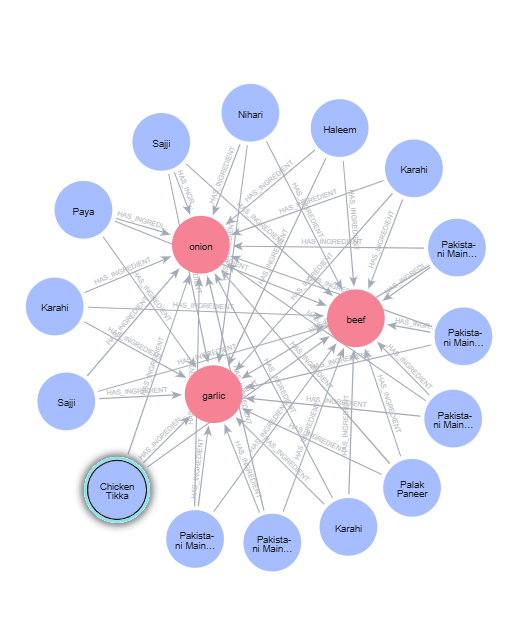
\includegraphics[width=0.75\linewidth]{RQ2 Visualisation.png}
    \caption{Neo4j graph visualization detailing a localized cluster of high-carbon co-occurrence. The graph highlights a central high-footprint \texttt{:Recipe} node connected via \texttt{HAS\_INGREDIENT} edges to multiple high-impact \texttt{:Ingredient} nodes (e.g., Mutton and Ghee). The visualization demonstrates how the graph architecture captures the compounding environmental impact when multiple emission-heavy ingredients are structurally linked within a single culinary instance.}
    \label{fig:neo4j_viz_rQ2}
\end{figure}

\begin{figure}[H]
    \centering
    \includegraphics[width=0.75\linewidth]{output.png}
    \caption{Top 20 co-occurring ingredient pairs within the top-500 high-carbon recipes, ranked by their average combined CO2e contribution (blue bars, left axis). The overlaid points (orange, right axis) indicate the absolute frequency of co-occurrence. The chart illustrates that the highest emitting pairs strictly involve combinations of ruminant meats (Beef, Mutton) and dairy (Ghee, Paneer), whereas highly frequent pairings (e.g., Beef and Onion) do not necessarily yield the absolute highest combined carbon cost.}
    \label{fig:RQ2_results}
\end{figure}
% TODO: RQ2 --- top-N co-occurring ingredient pairs and average CO2e among top-k high-carbon recipes.
\paragraph{Research Question 3:} Is there a nutritional trade-off associated with a recipe’s carbon footprint, and does user engagement reflect awareness of this environmental cost?\\

\noindent\textbf{Approach:} To answer RQ3, recipes were connected to their nutritional data through the \texttt{HAS\_NUTRITION} edge and each recipe was classified into a carbon tier. Instead of setting fixed thresholds, the query calculated quartile boundaries by sorting all \texttt{total\_co2e} values and extracting the 25th and 75th percentiles. Recipes below the 25th percentile were categorised as low carbon, those above the 75th percentile as high carbon, and the remainder as medium carbon. Each group was then aggregated in terms of average protein, fat, sugar, and calorie content, as well as average rating and review count.

\begin{lstlisting}[style=cypherstyle]
MATCH (r:Recipe)-[:HAS_NUTRITION]->(np:NutritionalProfile)
WITH collect(r.total_co2e) AS all_co2e, collect(r) AS recipes, collect(np) AS profiles
// Sort co2e values manually
UNWIND all_co2e AS val
WITH val, recipes, profiles
ORDER BY val
WITH collect(val) AS sorted_co2e, recipes, profiles
UNWIND range(0, size(recipes)-1) AS idx
WITH recipes[idx] AS r, profiles[idx] AS np, sorted_co2e
WITH r, np, sorted_co2e,
     sorted_co2e[toInteger(size(sorted_co2e)*0.75)] AS q75,
     sorted_co2e[toInteger(size(sorted_co2e)*0.25)] AS q25
WITH r, np,
     CASE
       WHEN r.total_co2e >= q75 THEN 'high'
       WHEN r.total_co2e <= q25 THEN 'low'
       ELSE 'medium'
     END AS carbon_group
RETURN carbon_group,
       count(r)                          AS recipe_count,
       round(avg(np.calories)*10)/10     AS avg_calories,
       round(avg(np.protein_g)*10)/10    AS avg_protein,
       round(avg(np.fat_g)*10)/10        AS avg_fat,
       round(avg(np.sugar_g)*10)/10      AS avg_sugar,
       round(avg(r.rating)*100)/100      AS avg_rating,
       round(avg(r.review_count)*10)/10  AS avg_reviews
ORDER BY carbon_group
\end{lstlisting}

\begin{figure}[H]
    \centering
    \includegraphics[width=0.60\textwidth]{figures/macronutrients.png}
    \caption{Macro-nutrients by carbon group. Protein more than doubles across tiers (16.3~g in low to 34.2~g in high), and fat follows the same direction (20.9~g to 27.0~g), consistent with higher meat and dairy content in high-carbon recipes. Calories and sugar are stable across all three groups.}
    \label{fig:macronutrients}
\end{figure}

\begin{figure}[H]
    \centering
    \includegraphics[width=0.60\linewidth]{figures/user_rating.png}
    \caption{User engagement by carbon group. Ratings (4.24, 4.25, 4.26) and review counts (2,497, 2,495, 2,511) show no meaningful difference across carbon tiers. As users rate low-carbon recipes just as highly as high-carbon ones, there is a clear case for introducing eco-scores to make carbon cost visible, and for prioritising low-carbon recipes in recommendations without any expected drop in user satisfaction.}
    \label{fig:user_rating}
\end{figure}
% TODO: RQ3 --- nutritional profile vs carbon footprint and relation to user engagement.



\section{Other important aspects of the dataset and knowledge graph}

\question{\subsubsection*{Are there important aspects of the dataset/knowledge graph highlighted by the frameworks of Pushkarna et al.\ \cite{pushkarna} and Paullada et al.\ \cite{Paullada}, which are not covered in the sections above?  If so, note them here.}}


\newpage
\bibliographystyle{plain}
\bibliography{datasheet}

\appendix

\section{Preprocessing Assumptions}
\label{app:assumptions}

The gram-weight grounding pipeline (Section 7.1, Stage 2) relies on a set of documented assumptions wherever the source data did not provide a directly usable value. These are listed here for transparency, as some are necessarily coarse.

\subsection{Generic gram-weight fallback defaults}

When the USDA SR Legacy table contained no portion entry for a given ingredient--unit combination, the following fixed gram weights were assumed per unit. These apply to roughly 30\% of rows (Tier~3) and are deliberately conservative.

\begin{center}
\begin{tabular}{ll}
\hline
\textbf{Unit} & \textbf{Assumed grams} \\
\hline
tablespoon (tbsp) & 15.0 \\
teaspoon (tsp) & 5.0 \\
cup & 240.0 \\
clove & 4.0 \\
medium / count\_medium & 100.0 \\
large & 150.0 \\
small & 60.0 \\
egg & 50.0 \\
fillet & 150.0 \\
``to taste'' / needed / optional & 5.0 \\
other (unparseable) & 100.0 \\
\hline
\end{tabular}
\end{center}

\subsection{``By taste'' and other non-quantitative quantities}

Irreducible qualitative quantities (``to taste'', ``as needed'', ``optional'') carry no numeric value. They were assigned a single conservative default of \textbf{5\,g} --- comparable to a teaspoon of a spice or seasoning, which is the most common context for such phrasing. This is the strongest assumption in the pipeline: it treats every ``to taste'' instance identically regardless of ingredient. The impact is limited because such quantities apply almost exclusively to low-mass seasonings (salt, spices) and were flagged in the \texttt{usda\_tier} column.

\subsection{Liquid density conversions (ml $\rightarrow$ g)}

Quantities given in millilitres were converted to grams using established food-science density values, since USDA SR Legacy does not encode an \texttt{ml} unit. Where no specific density applied, water density (1.0\,g/ml) was assumed.

\begin{center}
\begin{tabular}{ll}
\hline
\textbf{Ingredient (substring)} & \textbf{Density (g/ml)} \\
\hline
milk & 1.03 \\
cream & 1.01 \\
yogurt & 1.03 \\
ghee & 0.90 \\
butter & 0.91 \\
oil & 0.92 \\
water (default) & 1.00 \\
\hline
\end{tabular}
\end{center}

\subsection{Count-based unit remapping}

When an ingredient's quantity parsed to a generic ``other'' unit but the ingredient is naturally counted, the unit was remapped to a meaningful one before USDA lookup: \texttt{egg} $\rightarrow$ egg, \texttt{fish} $\rightarrow$ fillet, \texttt{lentils} / \texttt{lentils (dal)} $\rightarrow$ medium.

\subsection{Multi-entry disambiguation (plainness scoring)}

USDA SR Legacy often contains many entries for one base ingredient (e.g.\ beef appears as raw, stewed, dried, grilled). To select a representative gram weight, each candidate was scored by a \emph{plainness} heuristic: raw/fresh descriptions were rewarded; cooked, fried, salted, seasoned, sweetened, or all-caps-branded descriptions were penalised. The median gram weight of the five plainest matches was used. This assumes the raw, point-of-purchase ingredient state, which is the correct reference for LCA-based emission factors.

\section{Ingredient and Source Mappings}
\label{app:mappings}

This appendix records the manual mappings used to achieve 100\% CO$_2$e and gram-weight coverage. Some mappings are deliberate proxies: where no exact match existed in a reference dataset, the closest available category was chosen to guarantee full coverage. These approximations are noted explicitly, as they introduce a known, bounded source of error.

\subsection{Wolfram synonym map (\texttt{WOLFRAM\_MAP})}

Recipe ingredient names mapped to Wolfram canonical food names. Many are simple inflection matches to the Wolfram file's vocabulary (which pluralises most foods, e.g.\ almonds, cashews, cloves, chickpeas); others are deliberate proxies (e.g.\ ghee mapped to butter, garam masala mapped to the generic ``spice'' category).

\begin{center}
\begin{tabular}{ll|ll}
\hline
\textbf{Recipe name} & \textbf{Wolfram name} & \textbf{Recipe name} & \textbf{Wolfram name} \\
\hline
lentils (dal) & lentils & eggs & egg \\
mint leaves & fresh mint & fenugreek leaves & fenugreek seed \\
fresh coriander & coriander seed & curry leaves & curry powder \\
coriander & coriander seed & chickpeas & chickpeas \\
tamarind paste & tamarinds & fish & fishes \\
sesame seeds & sesames & mustard seeds & mustard \\
green chili & chili peppers & almonds & almonds \\
red chili powder & chili peppers & cashews & cashews \\
bell pepper & pepper & raisins & raisins \\
oil / cooking oil & sesame oil & bay leaf & herbs \\
all-purpose flour & wheat flour & peas & peas \\
garam masala & spice & ghee & butter \\
black pepper & black peppercorn & salt & sea salt \\
cloves & cloves & milk & milk \\
water & bottled water & carrot & carrots \\
cauliflower & cauliflowers & chicken & chickens \\
onion & onions & & \\
\hline
\end{tabular}
\end{center}

\noindent\textbf{Notable proxies / approximations:}
\begin{itemize}
    \item \textbf{ghee $\rightarrow$ butter:} ghee is clarified butter; the closest Wolfram entry, accepting that clarification alters mass slightly.
    \item \textbf{garam masala $\rightarrow$ spice} and \textbf{curry leaves $\rightarrow$ curry powder:} composite or leaf spices mapped to generic spice categories, as no exact entry exists.
    \item \textbf{fenugreek leaves $\rightarrow$ fenugreek seed:} the leaf form is absent; the seed is the only available proxy and may differ in emission intensity.
    \item \textbf{oil / cooking oil $\rightarrow$ sesame oil:} unspecified oil mapped to a concrete oil entry; actual cooking oils vary.
    \item \textbf{bay leaf $\rightarrow$ herbs} and \textbf{salt $\rightarrow$ sea salt:} broad-category proxies chosen to ensure coverage.
\end{itemize}

\subsection{OWID fallback map (\texttt{OWID\_MAP})}

Only 4 ingredients are absent from the Wolfram file (under any inflection); these draw their CO$_2$e value from OWID GHG categories.

\begin{center}
\begin{tabular}{ll}
\hline
\textbf{Recipe ingredient} & \textbf{OWID entity} \\
\hline
paneer & Cheese \\
semolina & Wheat \& Rye \\
potato & Potatoes \\
tomato & Tomatoes \\
\hline
\end{tabular}
\end{center}

\noindent\textbf{Notable proxies / approximations:} \textbf{paneer $\rightarrow$ Cheese} (paneer is a fresh cheese; the OWID Cheese category is a reasonable but not exact match, 23.88\,kg CO$_2$e/kg). \textbf{semolina $\rightarrow$ Wheat \& Rye} (OWID has no refined-semolina category; the whole-grain wheat category slightly overestimates emissions for refined semolina --- no closer category exists). \textbf{potato} and \textbf{tomato} map to their direct OWID production categories.

\subsection{USDA lookup synonyms (\texttt{USDA\_SYNONYMS})}

Where a recipe ingredient name would not match USDA SR Legacy descriptions directly, the following search keywords were substituted for the gram-weight lookup. A value of \emph{none} indicates the ingredient is absent from USDA and falls through to the generic gram-weight defaults.

\begin{center}
\begin{tabular}{ll|ll}
\hline
\textbf{Recipe ingredient} & \textbf{USDA keyword} & \textbf{Recipe ingredient} & \textbf{USDA keyword} \\
\hline
ghee & butter, salted & paneer & cottage cheese \\
garam masala & curry powder & fenugreek leaves & fenugreek \\
fresh coriander & coriander leaf & basmati rice & rice, white \\
mint leaves & spearmint & curry leaves & \emph{none} (generic) \\
lentils (dal) & lentils & carrot & carrots, raw \\
mustard seeds & mustard seed & green chili & peppers, chili \\
sesame seeds & sesame seed & bell pepper & peppers, sweet \\
tamarind paste & tamarind & & \\
\hline
\end{tabular}
\end{center}

\noindent\textbf{Approximations:} \textbf{ghee $\rightarrow$ ``butter, salted''} and \textbf{paneer $\rightarrow$ ``cottage cheese''} are mass proxies (no exact USDA entry); \textbf{garam masala $\rightarrow$ ``curry powder''} substitutes one spice blend for another; \textbf{curry leaves} has no USDA portion data and uses generic defaults.

\section{Client reflection on project outcomes}
\end{document}
